\begin{figure}[H]
    \centering
        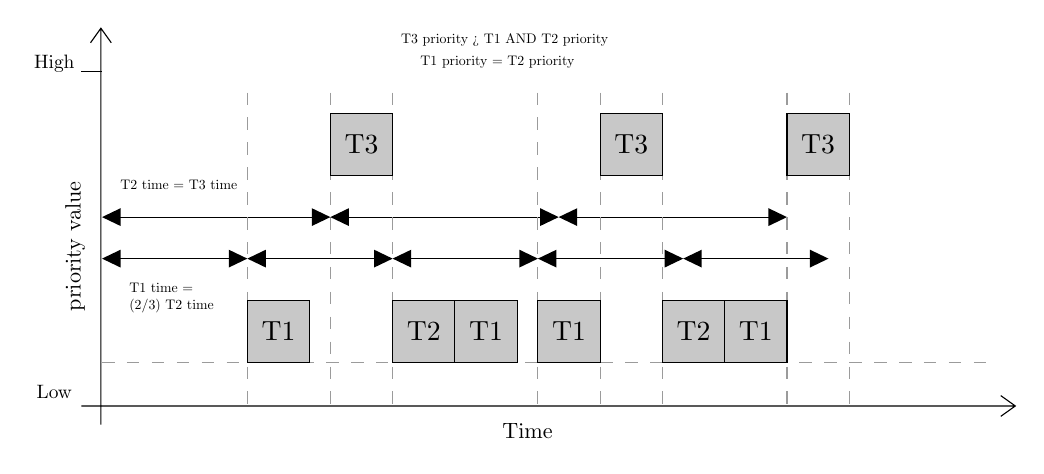
\begin{tikzpicture}[x=0.75pt,y=0.75pt,yscale=-1,xscale=1]
        \draw  (50,241) -- (500,241)(59.45,59) -- (59.45,250) (493,236) -- (500,241) -- (493,246) (54.45,66) -- (59.45,59) -- (64.45,66)  ;
        \draw    (50,80) -- (60,80) ;
        \draw [color={rgb, 255:red, 155; green, 155; blue, 155 }  ,draw opacity=1 ] [dash pattern={on 4.5pt off 4.5pt}]  (60,220) -- (490,220) ;
        \draw [color={rgb, 255:red, 155; green, 155; blue, 155 }  ,draw opacity=1 ] [dash pattern={on 4.5pt off 4.5pt}]  (170,90) -- (170,240) ;
        \draw    (62,170) -- (128,170) ;
        \draw [shift={(130,170)}, rotate = 180] [fill={rgb, 255:red, 0; green, 0; blue, 0 }  ][line width=0.75]  [draw opacity=0] (8.93,-4.29) -- (0,0) -- (8.93,4.29) -- cycle    ;
        \draw [shift={(60,170)}, rotate = 0] [fill={rgb, 255:red, 0; green, 0; blue, 0 }  ][line width=0.75]  [draw opacity=0] (8.93,-4.29) -- (0,0) -- (8.93,4.29) -- cycle    ;
        \draw  [fill={rgb, 255:red, 200; green, 200; blue, 200 }  ,fill opacity=1 ] (230,190) -- (260,190) -- (260,220) -- (230,220) -- cycle ;
        \draw    (62,150) -- (168,150) ;
        \draw [shift={(170,150)}, rotate = 180] [fill={rgb, 255:red, 0; green, 0; blue, 0 }  ][line width=0.75]  [draw opacity=0] (8.93,-4.29) -- (0,0) -- (8.93,4.29) -- cycle    ;
        \draw [shift={(60,150)}, rotate = 0] [fill={rgb, 255:red, 0; green, 0; blue, 0 }  ][line width=0.75]  [draw opacity=0] (8.93,-4.29) -- (0,0) -- (8.93,4.29) -- cycle    ;
        \draw    (172,150) -- (278,150) ;
        \draw [shift={(280,150)}, rotate = 180] [fill={rgb, 255:red, 0; green, 0; blue, 0 }  ][line width=0.75]  [draw opacity=0] (8.93,-4.29) -- (0,0) -- (8.93,4.29) -- cycle    ;
        \draw [shift={(170,150)}, rotate = 0] [fill={rgb, 255:red, 0; green, 0; blue, 0 }  ][line width=0.75]  [draw opacity=0] (8.93,-4.29) -- (0,0) -- (8.93,4.29) -- cycle    ;
        \draw    (282,150) -- (388,150) ;
        \draw [shift={(390,150)}, rotate = 180] [fill={rgb, 255:red, 0; green, 0; blue, 0 }  ][line width=0.75]  [draw opacity=0] (8.93,-4.29) -- (0,0) -- (8.93,4.29) -- cycle    ;
        \draw [shift={(280,150)}, rotate = 0] [fill={rgb, 255:red, 0; green, 0; blue, 0 }  ][line width=0.75]  [draw opacity=0] (8.93,-4.29) -- (0,0) -- (8.93,4.29) -- cycle    ;
        \draw [color={rgb, 255:red, 155; green, 155; blue, 155 }  ,draw opacity=1 ] [dash pattern={on 4.5pt off 4.5pt}]  (270,90) -- (270,240) ;
        \draw [color={rgb, 255:red, 155; green, 155; blue, 155 }  ,draw opacity=1 ] [dash pattern={on 4.5pt off 4.5pt}]  (390,90) -- (390,240) ;
        \draw [color={rgb, 255:red, 155; green, 155; blue, 155 }  ,draw opacity=1 ] [dash pattern={on 4.5pt off 4.5pt}]  (200,90) -- (200,240) ;
        \draw [color={rgb, 255:red, 155; green, 155; blue, 155 }  ,draw opacity=1 ] [dash pattern={on 4.5pt off 4.5pt}]  (130,90) -- (130,240) ;
        \draw [color={rgb, 255:red, 155; green, 155; blue, 155 }  ,draw opacity=1 ] [dash pattern={on 4.5pt off 4.5pt}]  (300,90) -- (300,240) ;
        \draw    (132,170) -- (198,170) ;
        \draw [shift={(200,170)}, rotate = 180] [fill={rgb, 255:red, 0; green, 0; blue, 0 }  ][line width=0.75]  [draw opacity=0] (8.93,-4.29) -- (0,0) -- (8.93,4.29) -- cycle    ;
        \draw [shift={(130,170)}, rotate = 0] [fill={rgb, 255:red, 0; green, 0; blue, 0 }  ][line width=0.75]  [draw opacity=0] (8.93,-4.29) -- (0,0) -- (8.93,4.29) -- cycle    ;
        \draw    (202,170) -- (268,170) ;
        \draw [shift={(270,170)}, rotate = 180] [fill={rgb, 255:red, 0; green, 0; blue, 0 }  ][line width=0.75]  [draw opacity=0] (8.93,-4.29) -- (0,0) -- (8.93,4.29) -- cycle    ;
        \draw [shift={(200,170)}, rotate = 0] [fill={rgb, 255:red, 0; green, 0; blue, 0 }  ][line width=0.75]  [draw opacity=0] (8.93,-4.29) -- (0,0) -- (8.93,4.29) -- cycle    ;
        \draw    (272,170) -- (338,170) ;
        \draw [shift={(340,170)}, rotate = 180] [fill={rgb, 255:red, 0; green, 0; blue, 0 }  ][line width=0.75]  [draw opacity=0] (8.93,-4.29) -- (0,0) -- (8.93,4.29) -- cycle    ;
        \draw [shift={(270,170)}, rotate = 0] [fill={rgb, 255:red, 0; green, 0; blue, 0 }  ][line width=0.75]  [draw opacity=0] (8.93,-4.29) -- (0,0) -- (8.93,4.29) -- cycle    ;
        \draw    (342,170) -- (408,170) ;
        \draw [shift={(410,170)}, rotate = 180] [fill={rgb, 255:red, 0; green, 0; blue, 0 }  ][line width=0.75]  [draw opacity=0] (8.93,-4.29) -- (0,0) -- (8.93,4.29) -- cycle    ;
        \draw [shift={(340,170)}, rotate = 0] [fill={rgb, 255:red, 0; green, 0; blue, 0 }  ][line width=0.75]  [draw opacity=0] (8.93,-4.29) -- (0,0) -- (8.93,4.29) -- cycle    ;
        \draw  [fill={rgb, 255:red, 200; green, 200; blue, 200 }  ,fill opacity=1 ] (270,190) -- (300,190) -- (300,220) -- (270,220) -- cycle ;
        \draw [color={rgb, 255:red, 155; green, 155; blue, 155 }  ,draw opacity=1 ] [dash pattern={on 4.5pt off 4.5pt}]  (330,90) -- (330,240) ;
        \draw  [fill={rgb, 255:red, 200; green, 200; blue, 200 }  ,fill opacity=1 ] (300,100) -- (330,100) -- (330,130) -- (300,130) -- cycle ;
        \draw  [fill={rgb, 255:red, 200; green, 200; blue, 200 }  ,fill opacity=1 ] (170,100) -- (200,100) -- (200,130) -- (170,130) -- cycle ;
        \draw  [fill={rgb, 255:red, 200; green, 200; blue, 200 }  ,fill opacity=1 ] (200,190) -- (230,190) -- (230,220) -- (200,220) -- cycle ;
        \draw [color={rgb, 255:red, 155; green, 155; blue, 155 }  ,draw opacity=1 ] [dash pattern={on 4.5pt off 4.5pt}]  (420,90) -- (420,240) ;
        \draw  [fill={rgb, 255:red, 200; green, 200; blue, 200 }  ,fill opacity=1 ] (330,190) -- (360,190) -- (360,220) -- (330,220) -- cycle ;
        \draw  [fill={rgb, 255:red, 200; green, 200; blue, 200 }  ,fill opacity=1 ] (390,100) -- (420,100) -- (420,130) -- (390,130) -- cycle ;
        \draw  [fill={rgb, 255:red, 200; green, 200; blue, 200 }  ,fill opacity=1 ] (130,190) -- (160,190) -- (160,220) -- (130,220) -- cycle ;
        \draw  [fill={rgb, 255:red, 200; green, 200; blue, 200 }  ,fill opacity=1 ] (360,190) -- (390,190) -- (390,220) -- (360,220) -- cycle ;
        \draw (47,164) node [scale=0.8,rotate=-270] [align=left] {priority value};
        \draw (265,253) node [scale=0.8] [align=left] {Time};
        \draw (37,76) node [scale=0.7] [align=left] {High};
        \draw (37,234) node [scale=0.7] [align=left] {Low};
        \draw (245,205) node  [align=left] {T1};
        \draw (185,115) node  [align=left] {T3};
        \draw (215,205) node  [align=left] {T2};
        \draw (285,205) node  [align=left] {T1};
        \draw (315,115) node  [align=left] {T3};
        \draw (405,115) node  [align=left] {T3};
        \draw (145,205) node  [align=left] {T1};
        \draw (97,134.5) node [scale=0.5] [align=left] {T2 time = T3 time};
        \draw (254,64.5) node [scale=0.5] [align=left] {T3 priority > T1 AND T2 priority};
        \draw (250.5,75.5) node [scale=0.5] [align=left] {T1 priority = T2 priority};
        \draw (93.5,189) node [scale=0.5] [align=left] {T1 time = \\(2/3) T2 time};
        \draw (345,205) node  [align=left] {T2};
        \draw (375,205) node  [align=left] {T1};
    \end{tikzpicture}
    \caption{Priority scheduling example with three (3) tasks attached triggered by time-elapsed events}
    \label{fig:timelapsed}
\end{figure}
